%%%%%%%%%%%%%%%%%%%%%%% file typeinst.tex %%%%%%%%%%%%%%%%%%%%%%%%%
%
% This is the LaTeX source for the instructions to authors using
% the LaTeX document class 'llncs.cls' for contributions to
% the Lecture Notes in Computer Sciences series.
% http://www.springer.com/lncs       Springer Heidelberg 2006/05/04
%
% It may be used as a template for your own input - copy it
% to a new file with a new name and use it as the basis
% for your article.
%
% NB: the document class 'llncs' has its own and detailed documentation, see
% ftp://ftp.springer.de/data/pubftp/pub/tex/latex/llncs/latex2e/llncsdoc.pdf
%
%%%%%%%%%%%%%%%%%%%%%%%%%%%%%%%%%%%%%%%%%%%%%%%%%%%%%%%%%%%%%%%%%%%


\documentclass[runningheads,a4paper]{llncs}

\usepackage{amssymb}
\setcounter{tocdepth}{3}
\usepackage{graphicx}
\usepackage{hyperref}
\usepackage{amsmath}
\usepackage{listings}

\usepackage{tikz}
\usetikzlibrary{positioning,arrows,shapes.geometric,
	matrix,shapes.symbols,decorations.pathreplacing}

\usepackage{subcaption}
\captionsetup{compatibility=false}

\usepackage{booktabs}

\usepackage[utf8]{inputenc}
\usepackage[T1]{fontenc}
\usepackage{lmodern}

\usepackage{url}
\urldef{\mailsa}\path|loic_tetrel@yahoo.fr|
\newcommand{\keywords}[1]{\par\addvspace\baselineskip
	\noindent\keywordname\enspace\ignorespaces#1}

\begin{document}
	
	\mainmatter  % start of an individual contribution
	
	% first the title is needed
	\title{Bayesian Model for Machine Learning}
	
	% a short form should be given in case it is too long for the running head
	\titlerunning{Bayesian Model for Machine Learning}%
	
	% the name(s) of the author(s) follow(s) next
	%
	% NB: Chinese authors should write their first names(s) in front of
	% their surnames. This ensures that the names appear correctly in
	% the running heads and the author index.
	%
	\author{Loïc Tetrel}
	%
	\authorrunning{Bayesian Model for Machine Learning}
	% (feature abused for this document to repeat the title also on left hand pages)
	
	% the affiliations are given next; don't give your e-mail address
	% unless you accept that it will be published
	%\institute{******************************************\\
	\institute{}
	
	%
	% NB: a more complex sample for affiliations and the mapping to the
	% corresponding authors can be found in the file "llncs.dem"
	% (search for the string "\mainmatter" where a contribution starts).
	% "llncs.dem" accompanies the document class "llncs.cls".
	%
	
	\toctitle{Bayesian Model for Machine Learning}
	
	\maketitle

	\keywords{Generative model; Bayes; Prediction}

	\section{Introduction}\label{introduction}
	Thomas Bayes is a well known mathematician, with work focused in probability. Bayes theory\cite{bayes1958essay} is central in machine learning and has numerous applications in automatic classification.
	
	\section{Theory}\label{theory}
	Consider two event $a$ and $b$, the Bayesian rule define the probability $P$ that $a$ occurs, knowing the result of the event $b$ :
	
	\begin{equation}
	P(a|b) = \frac{P(b|a) \times P(a)}{P(b)} 
	\end{equation}
	
	It can be interpreted as is : if we know a priori the probabilities of the events $a$, $b$, and the result of the event $b$ (knowing result of $a$), then we can deduct the result $a$ (knowing result of $b$). \\ Using this rule will allow us to infer things about the income of events, when you have some aprioris. This is the base in Machine Learning, with training data, you infer the result for testing data.
		
	\section{Code example}\label{example}
	Let's do a practical example of what Bayes is. Imagine you are in charge of a production line, this line sort strawberries from grapes. To do this, you bought cameras and measure the radius of the fruits coming from the farmers. Your hypothesis is that the radius is a good predictor, and you want to use a bayesian rule to classify the fruits !
	
	\begin{equation}
	P(\omega_i|X) = \frac{P(X|\omega_i) \times P(\omega_i)}{P(X)} 
	\end{equation}
	
	Where $\omega_i = {\omega_g, \omega_c}$ are the events for $\omega_g$ : "The fruit is a grape", and $\omega_c$ "The fruit is a cherry". The measured radius is called $X$, $P(\omega_i)$ and $P(X)$ are called marginal probabilities, and $P(X|\omega_i)$ is known as the likelihood. One can define the likelihhod as : \textit{The probabilities of the incoming data, as if they belong to the classes}.
	
	\par
	First, you want to model the distribution of your fruits. In Machine learning, we usually refer the probability as a function called pdf (probability density function). A gaussian prior is often used. So you start acquiring many data while knowing what fruit it is, and calculate the parameters ($\mu$, $\sigma$) of the associated gaussian \footnote{Usually you want to calculate the likelihood of your data to verify if it's truly gaussian, or use a test like Student's t-test.}.
	
	\begin{lstlisting}[language=python]
	# Creation of data
	RadiusCherries = np.random.normal(4, 0.5, 1000)
	RadiusGrapes = np.random.normal(2, 0.5, 1000)
	
	# Estimators for gaussian mean and deviation
	MeanCherries = np.median(RadiusCherries)
	DevCherries = np.std(RadiusCherries)
	MeanGrapes = np.median(RadiusGrapes)
	DevGrapes = np.std(RadiusGrapes)
	\end{lstlisting}
	
	\begin{figure}
	\centering
	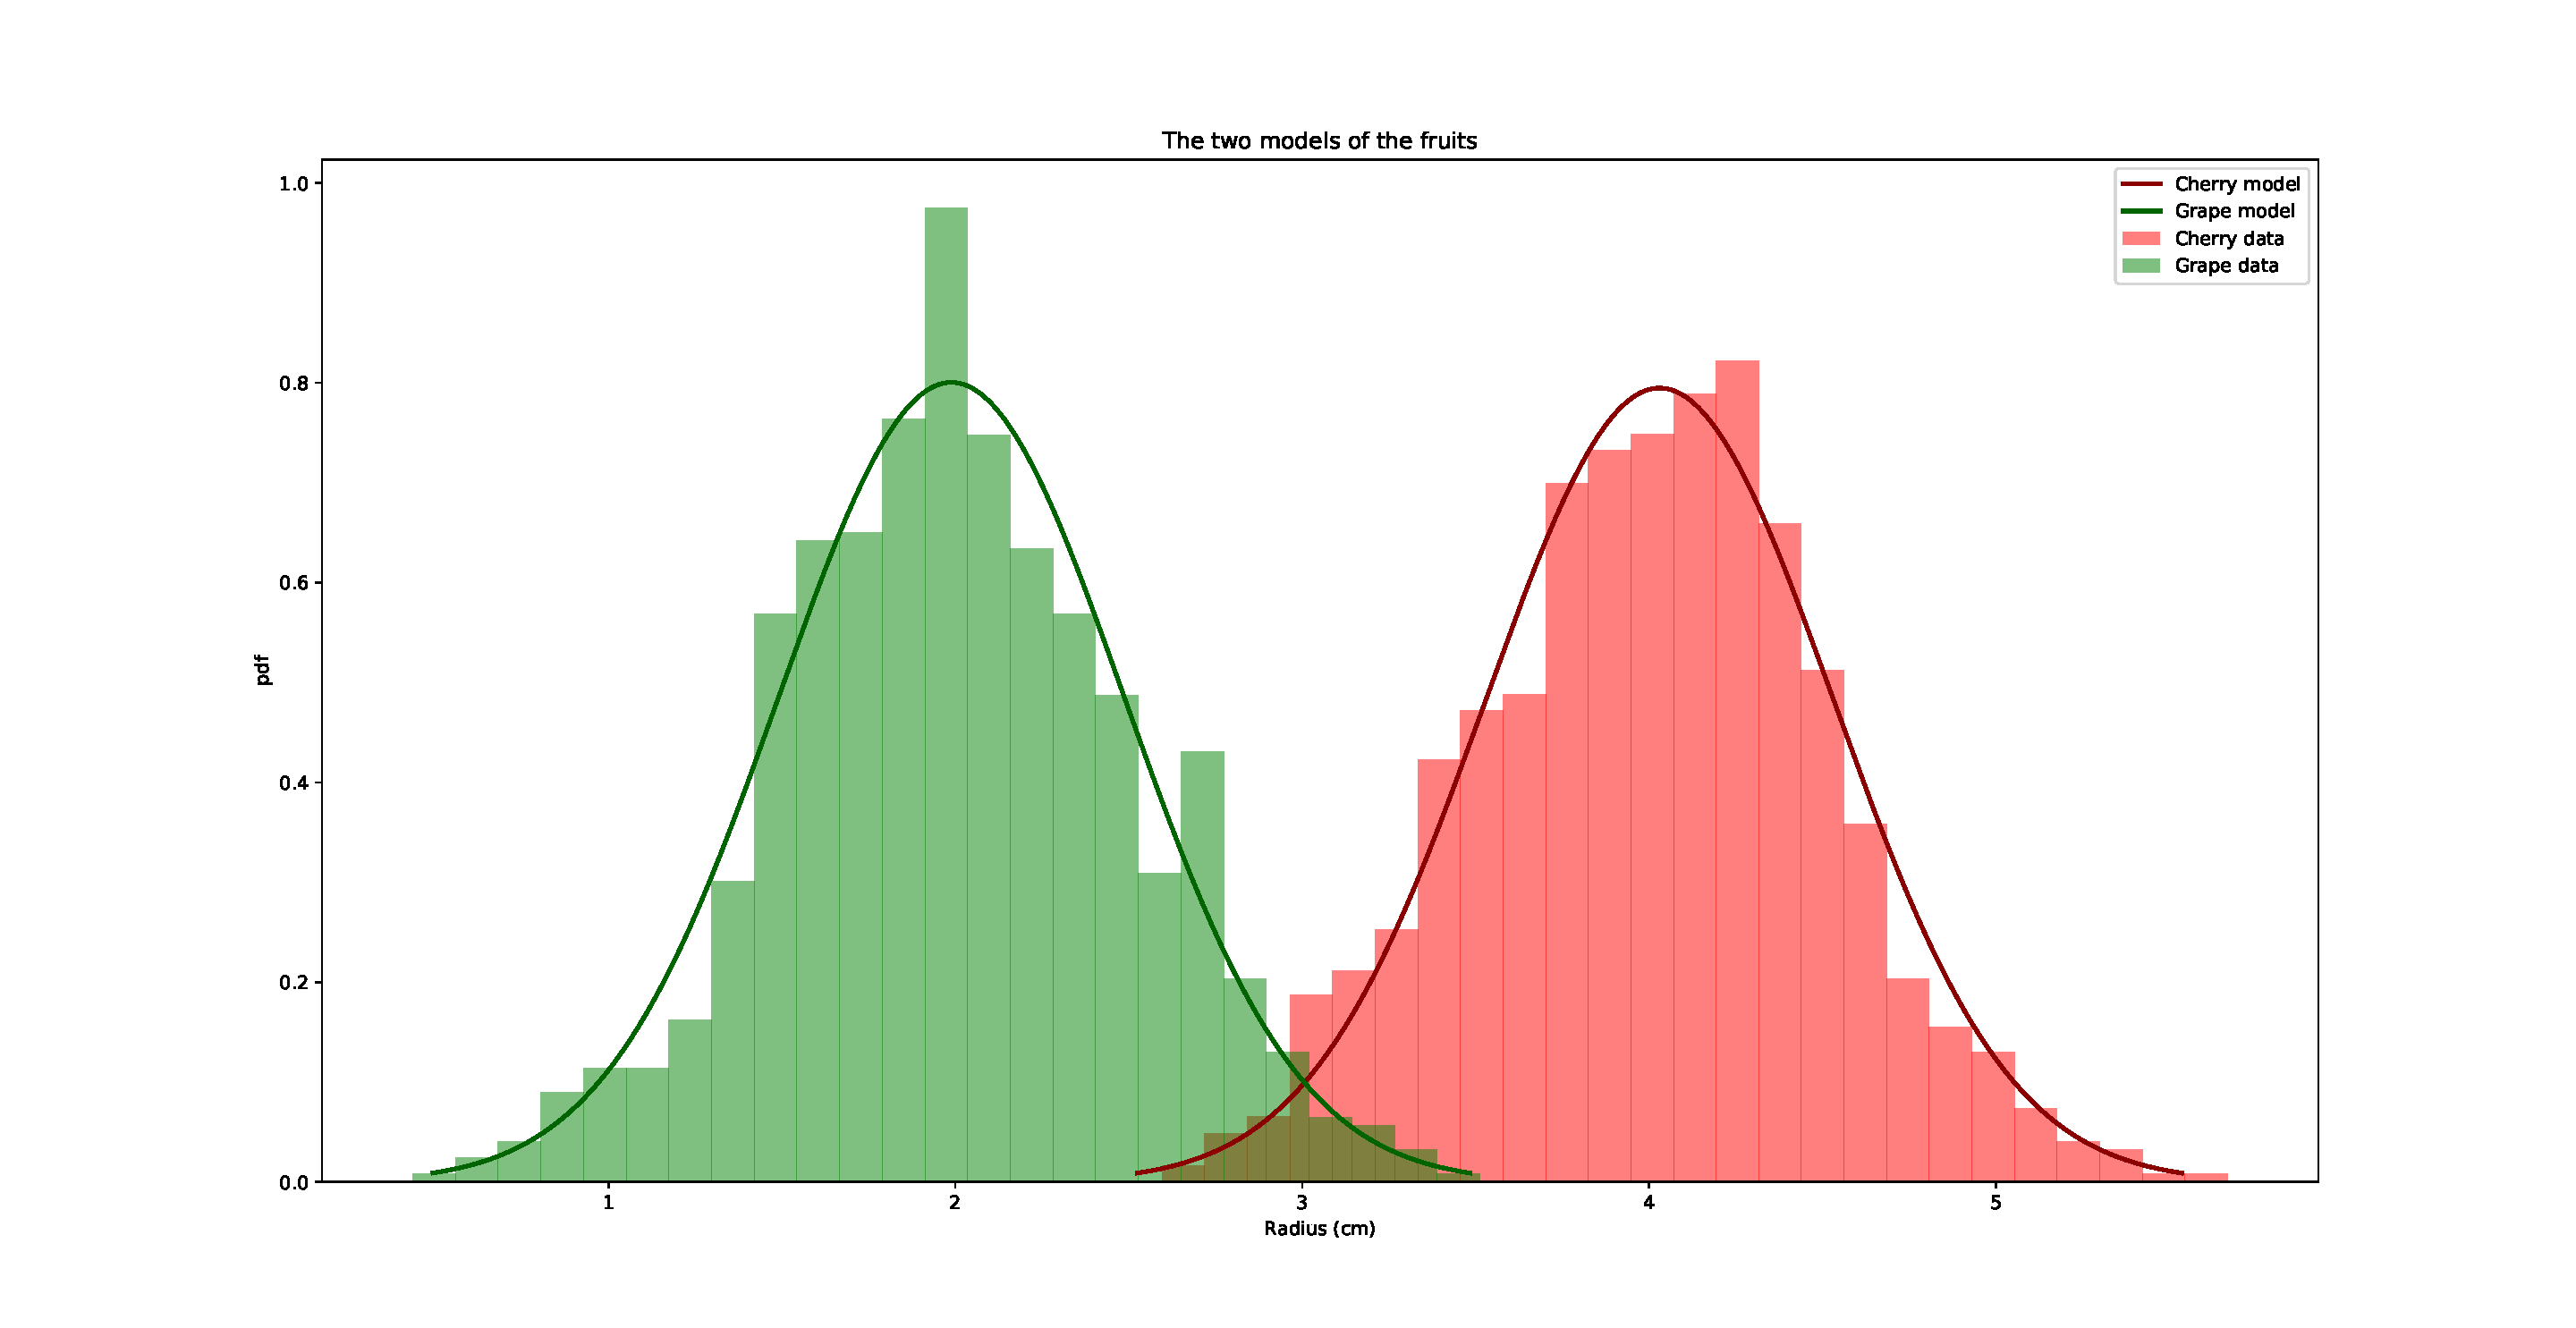
\includegraphics[width=0.75\textwidth]{Figures/distrib}
	\\ \parbox{0.75\textwidth}{\caption[Distribution]{The two models for the fruits.}\label{fig:distrib}} 
	\end{figure}
	
	Now that we have our models, we can evaluate the likelihood of the data for our classes. 
	\begin{lstlisting}[language=python]
	#New radius data coming in
	Data = np.array([1.52, 2.68, 3, 4, 6])
	
	#Bayes
	# P(w_c) = P(w_g)
	PAprioriCherry = PAprioriGrape = 0.5
	PData = 1
	LikelihoodsCherry = stats.norm(MeanCherries, DevCherries).pdf(Data)
	LikelihoodsGrape = stats.norm(MeanGrapes, DevGrapes).pdf(Data)
	\end{lstlisting}
	
	For example, the likelihood of $x = 3$ gives the figure \ref{fig:likelihood}.
	
	\begin{figure}
		\centering
		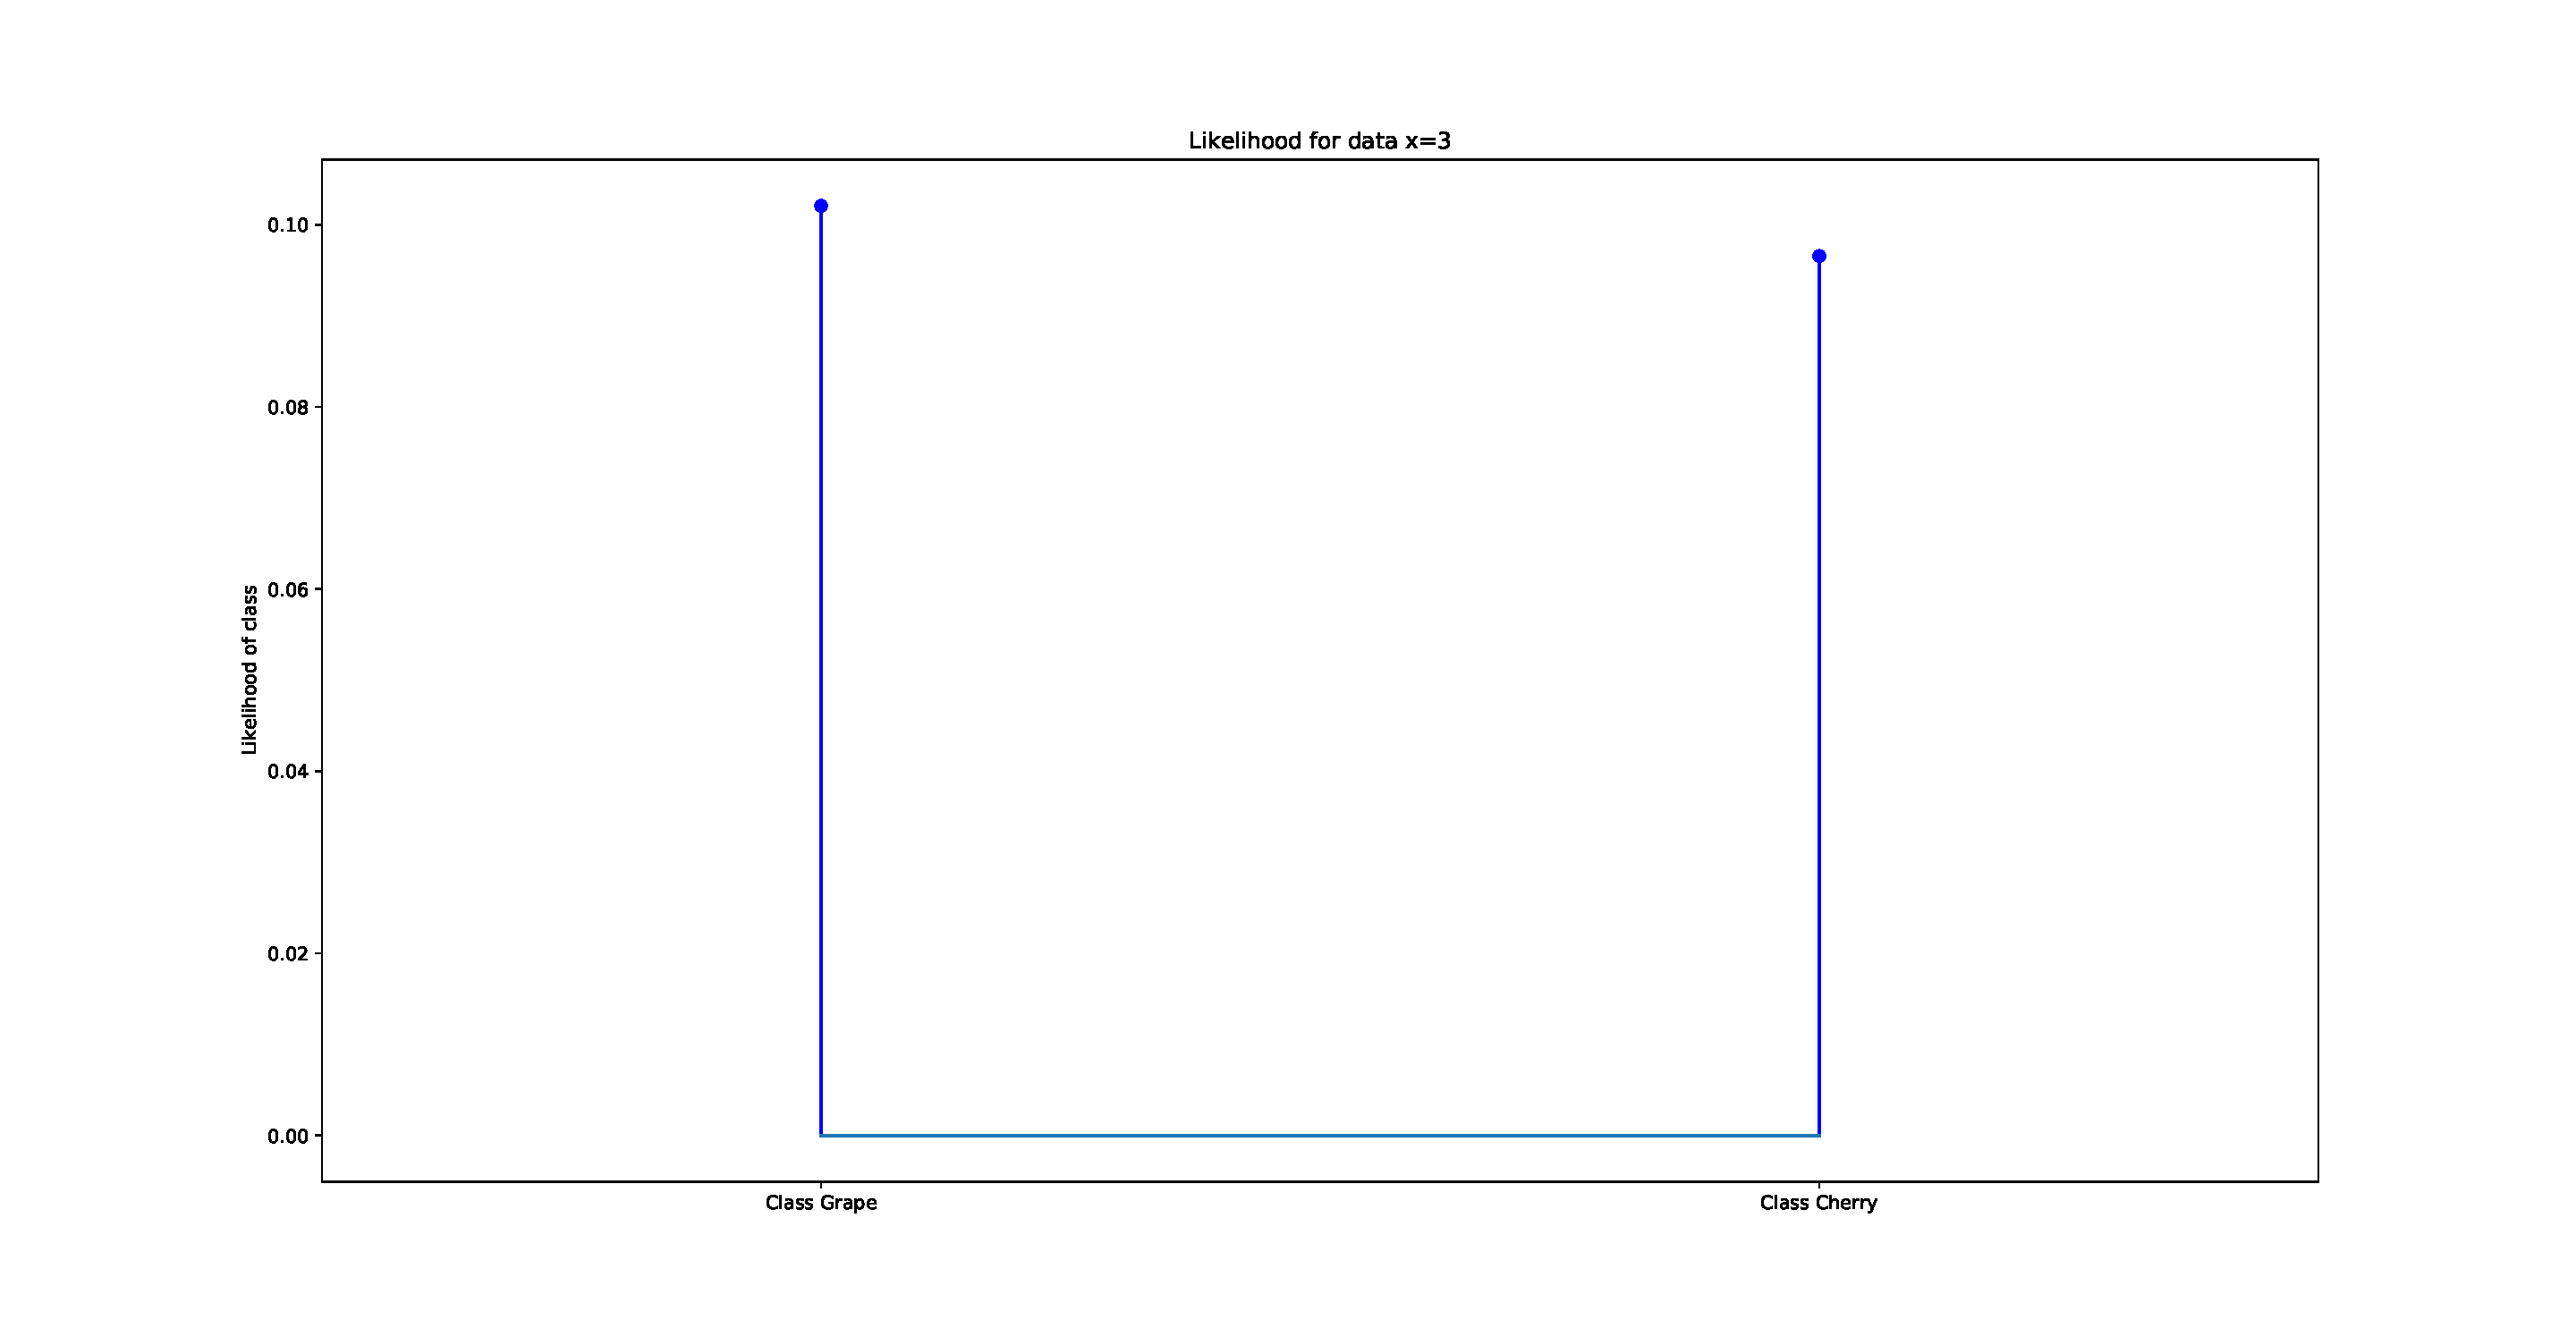
\includegraphics[width=0.75\textwidth]{Figures/likelihood}
		\\ \parbox{0.75\textwidth}{\caption[Likelihood]{Likelihood for one data.}\label{fig:likelihood}} 
	\end{figure}
	
	Now, we can evaluate the posterior probability (predict what type of fruit it is), given the marginals and the likelihood \footnote{Sometimes, it can be simpler and faster to evaluate just the likelihoods to do predictions.}.
	
	\begin{lstlisting}[language=python]
	PCherry = LikelihoodsCherry * PAprioriCherry/PData
	PGrape = LikelihoodsGrape * PAprioriGrape/PData
	\end{lstlisting}
	
	After we calculated the posterior for every data, the MAP (maximum aposteriori prediction) can be used to find to which class our measure comes from \ref{fig:preds}. So if $P(\omega_g|X) > P(\omega_c|X)$  that means that the data $X$ is more likely to be a grape.
	
	\begin{lstlisting}[language=python]
	for i in range(0, len(Data)):
	if PGrape[i] > PCherry[i]:
	plt.plot(Data[i], 0.02, 'o', color='darkgreen', linewidth=10, markersize=12)
	else:
	plt.plot(Data[i], 0.02, 'o', color='darkred', linewidth=10, markersize=12)
	\end{lstlisting}
	
	Be careful if the two probabilities are really close (in our example the 3rd fruit). In this case, you could use an uncertainty factor and decide to not predict it (it's ok, just throw this fruit !).
	
	\begin{figure}
	\centering
	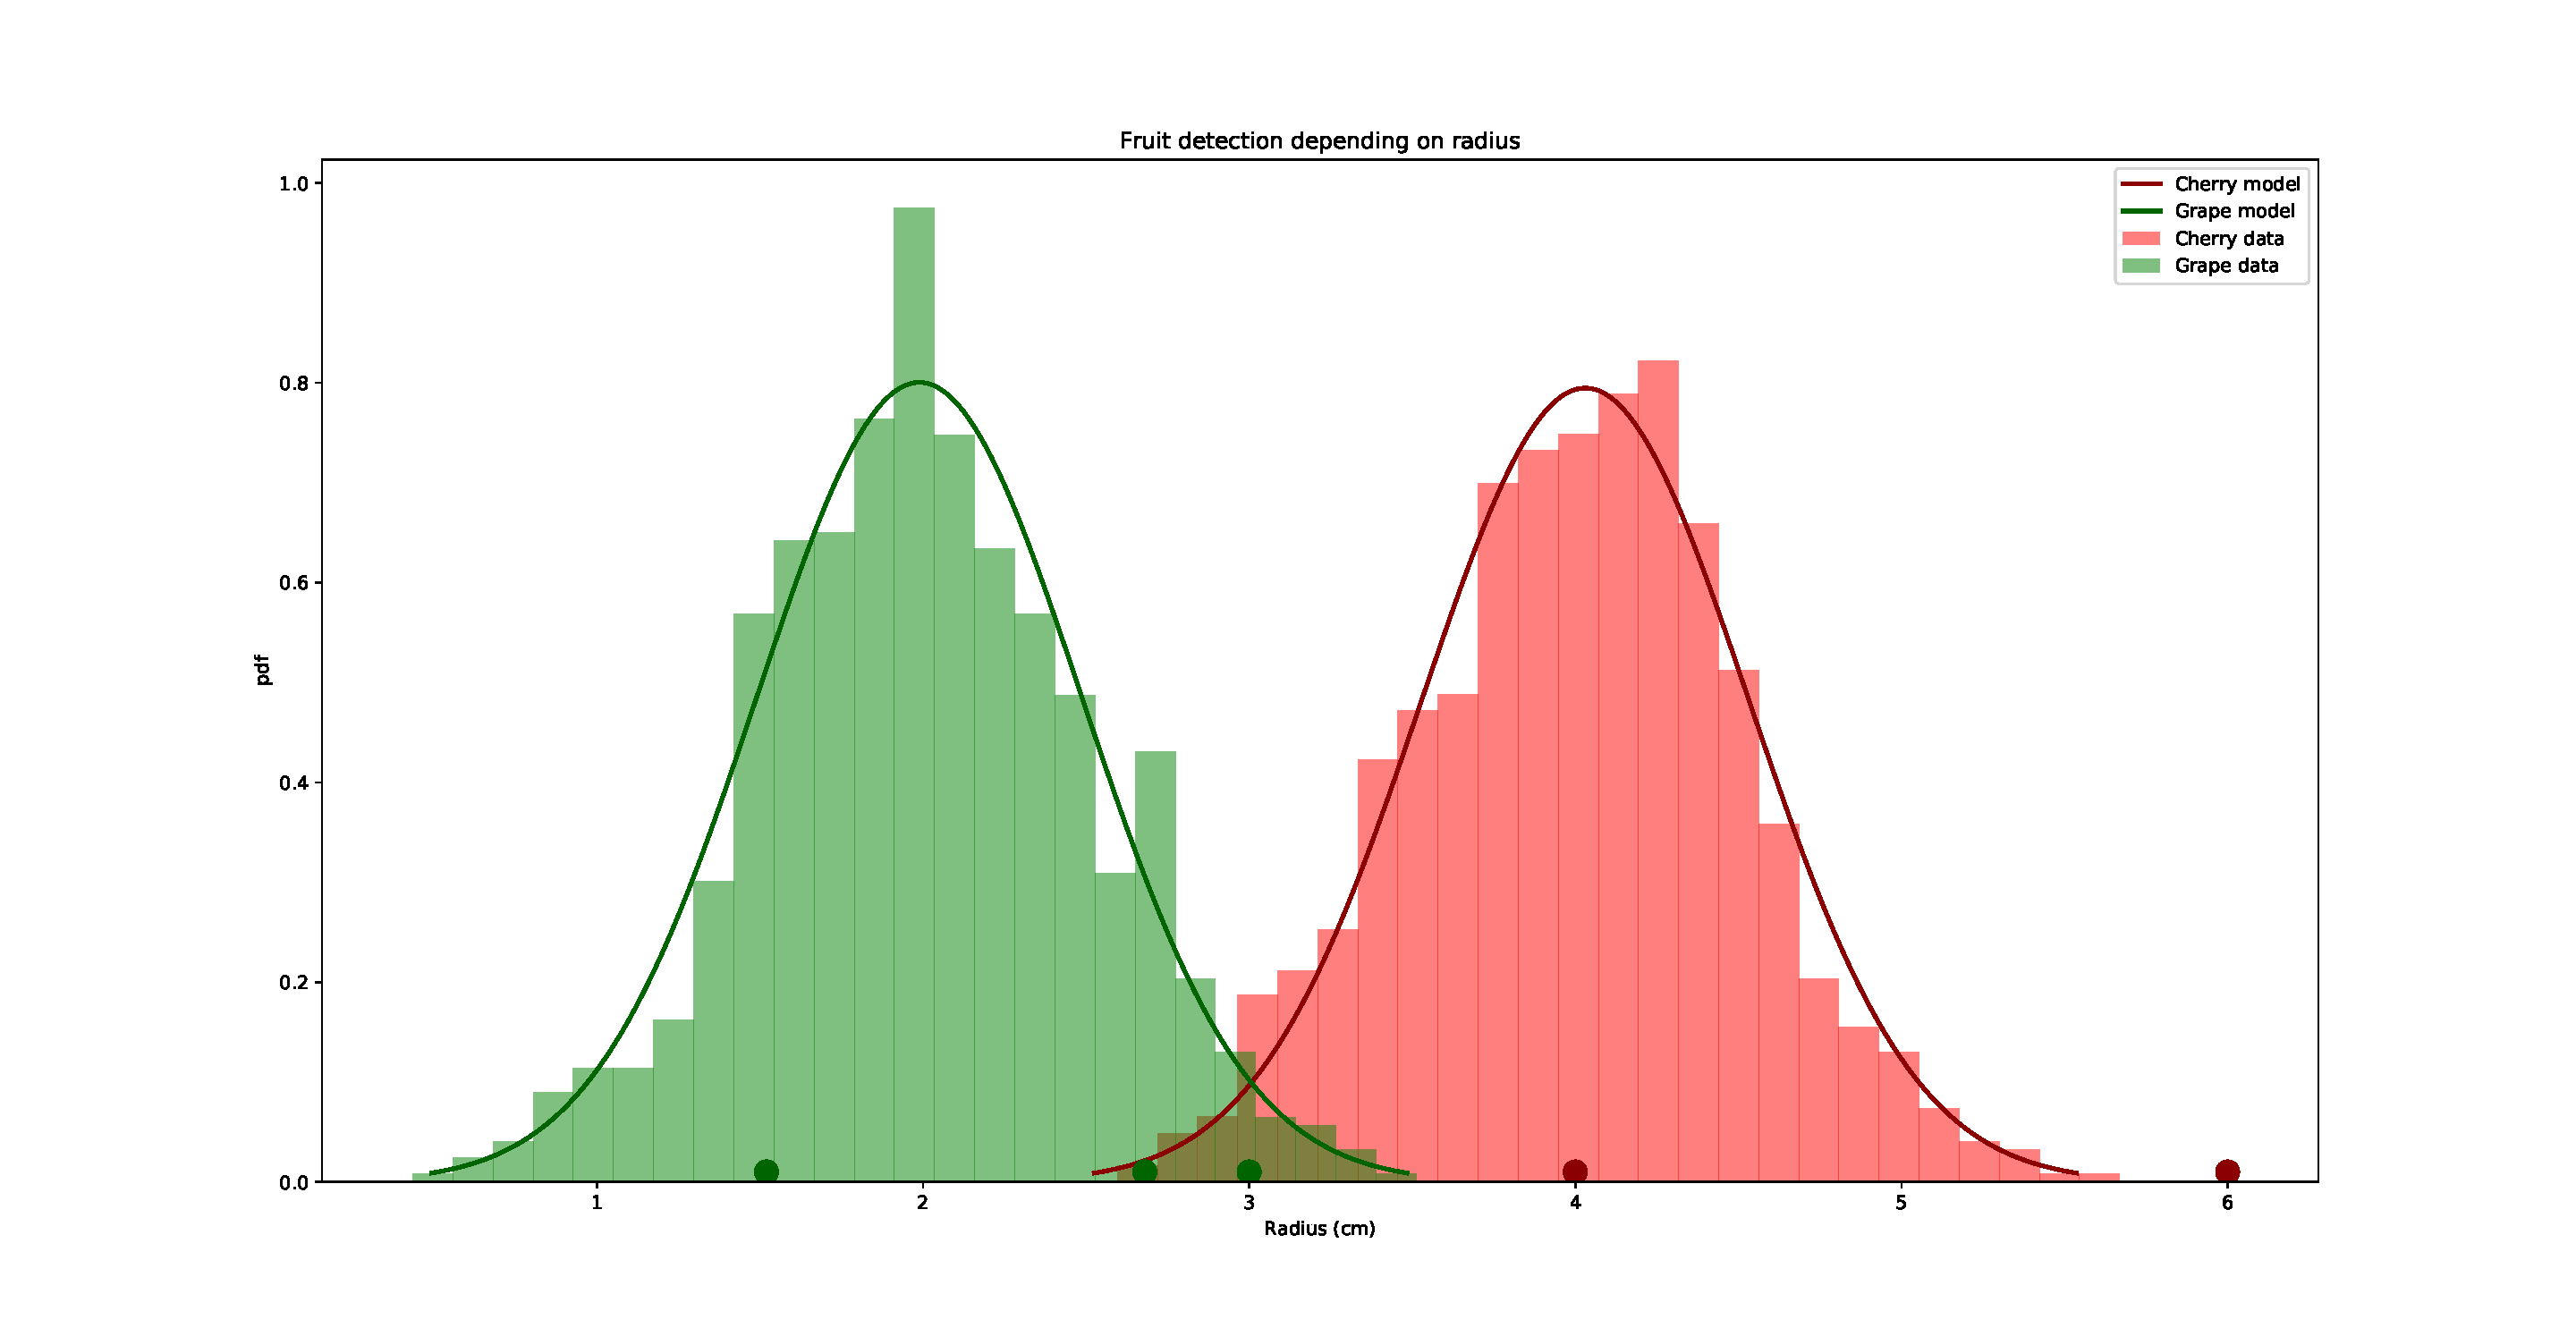
\includegraphics[width=0.75\textwidth]{Figures/preds}
	\\ \parbox{0.75\textwidth}{\caption[Distribution]{The prediction of $5$ fruits.}\label{fig:preds}} 
	\end{figure}
	
	\lstinputlisting[language=python]{BayesModel.py}
	
	\section{Study case}
	\label{sec:method}
	
	\section{Conclusion}
	\label{sec:conclusion}
	Example of Monty Hall problem, resolved using bayesian rule :
	\url{https://www.quora.com/How-do-I-solve-the-Monty-Hall-Problem-using-Bayes-Theorem}
	 
	\subsection*{Acknowledgment}
	Thanks
	
	{\small
		\bibliographystyle{splncs03}
		\bibliography{article}
	}
	
\end{document}

